\section{The band between the two thresholds}
\label{sec:band}

\subsection{One state in the band}

Take the best Gaussian state of the pendulum at $\sigma_0 = 0.1$, whose critical rate is $R(0) = 0.9081$, and blur it at $r = 0.9541 = (\kappa + R(0))/2$, in the middle of the band~\eqref{eq:band}. Figure~\ref{fig:band} shows both thresholds for this one state.

\emph{(I)} The forward SDE~\eqref{eq:sde}, run with the positive part $G_+$ of $G$, departs from the true law: the error of the variance along the most stretching direction grows steadily to $6\%$ at $t = 1$. At $r = 1$ and $1.1$ it stays below $1\%$, the remainder of the expansion behind Eq.~\eqref{eq:G}.

\emph{(II)} The coarse-grained entropy, measured directly with the nearest-neighbour estimator, grows exactly as predicted: by $0.363$ over $0 \leq t \leq 1$, against $0.363$ predicted. Meanwhile $R(t)$ falls from $0.908$ to $0.272$ as the state leaves the top, so the entropy grows faster and faster.

In this state the arrow of time is present, and visible to a learned score, while the noisy physical dynamics that would produce the blur does not exist.

\begin{figure*}[t]
\centering
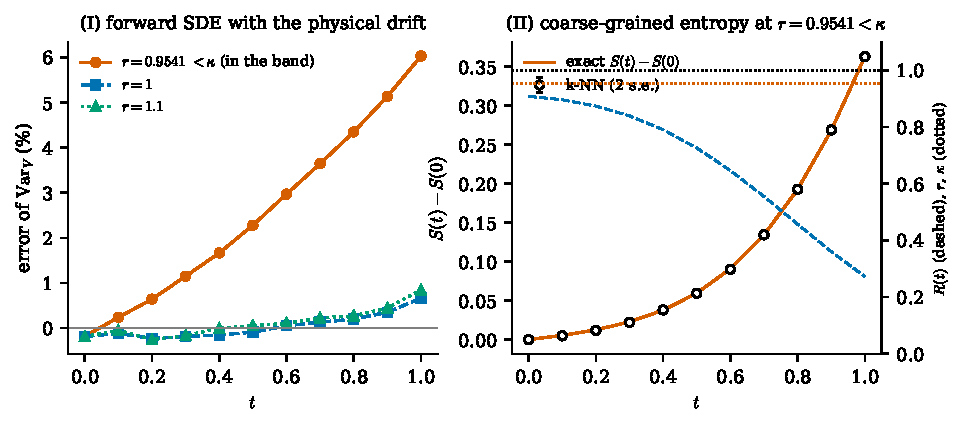
\includegraphics[width=0.9\textwidth]{figures/fig4_band.pdf}
\caption{One state in the band: pendulum, best Gaussian state, $\sigma_0 = 0.1$, $r = 0.9541$, between $R(0) = 0.9081$ and $\kappa = 1$. Left, threshold (I): relative error of the variance along the most stretching direction for the forward SDE with the physical drift and the clipped diffusion $G_+$; for comparison $r = 1$ and $1.1$. Right, threshold (II): entropy increase, exact (line) and measured with the nearest-neighbour estimator (circles, two standard errors); dashed, right axis: the critical rate $R(t)$; dotted: $r$ and $\kappa$.}
\label{fig:band}
\end{figure*}

\subsection{Where threshold (I) breaks}

To locate threshold (I) we scan $r/\kappa$ from $0.6$ to $1.3$ and measure, at the final time, the relative error of the variance along the most stretching direction (Fig.~\ref{fig:knee}). For the forward SDE we compare with the exact law. For the reverse direction we start from exact samples at the final time and run back both the reverse SDE with $G_+$ and the probability-flow equation, which needs no positive diffusion, with the same starting points; the difference isolates the effect of the missing diffusion. In four dimensions $\Sym Df$ depends on $q$, and $G$ is clipped pointwise: $G = U\operatorname{diag}(g)U^{\mathsf T}$, $G_+ = U\operatorname{diag}(\max(g,0))U^{\mathsf T}$.

\begin{observation}
\label{obs:knee}
In two and four dimensions, for $\sigma_0$ from $0.03$ to $0.3$ and with exact as well as learned scores, the error stays on a nearly flat plateau for $r \geq \kappa$ and grows as soon as $r < \kappa$. The learned score reproduces the curves of the exact score.
\end{observation}

The onset at $r = \kappa$ is exact: clipping happens only where $\lambda(q) > r$, which never occurs for $r \geq \kappa$ (Proposition~\ref{prop:sde}). Below $\kappa$ the error does not jump; it grows like a convex function of $\kappa - r$. If the curve is summarised by the zero of a straight line fitted through $r/\kappa = 0.8$, $0.9$ and $0.95$, this ``knee'' lies slightly below $\kappa$, further below for larger $\sigma_0$ and in four dimensions (Table~\ref{tab:knee}).

The shift has a simple origin. Clipping removes the diffusion $\sigma^2(\lambda - r)_+$ along the stretching direction, and only where the state has mass with $\lambda > r$. The total missing diffusion,
\begin{equation}
D(r) = \frac{1}{\sigma(T)^2}\int_0^T \E\big[\sigma(t)^2\,(\lambda(Y_t) - r)_+\big]\,dt ,
\label{eq:missing}
\end{equation}
vanishes for $r \geq \kappa$ and is convex below it, because a slightly smaller $r$ exposes only a small part of the state near the top. Applying the same straight-line rule to $D(r)$ gives a \emph{shape prediction} of the knee that uses no simulation of the SDE. It agrees with the measured knees to within $0.03$, and reproduces the trend with $\sigma_0$ and dimension (Table~\ref{tab:knee}). A wider state has more mass away from the top, so its exposure grows more slowly as $r$ decreases, and its knee lies further below $\kappa$. The knee is a property of the fit; the threshold is at $\kappa$.

\begin{table}[t]
\caption{Knee of threshold (I): zero of the straight line through $r/\kappa = 0.8$, $0.9$, $0.95$ of the difference between the reverse SDE and the probability-flow equation. Shape prediction: the same rule applied to the missing diffusion~\eqref{eq:missing}. Four dimensions: coupled pendulums, $\varepsilon = 0.3$.}
\label{tab:knee}
\begin{ruledtabular}
\begin{tabular}{ccccc}
dim. & $\sigma_0$ & exact score & learned score & shape \\
\hline
2 & $0.03$ & $1.005$ & $1.005$ & $0.987$ \\
2 & $0.1$ & $0.991$ & $0.990$ & $0.977$ \\
2 & $0.3$ & $0.972$ & $0.972$ & $0.965$ \\
4 & $0.1$ & $0.977$ & $0.960$ & $0.958$ \\
4 & $0.3$ & $0.978$ & $0.944$ & $0.951$ \\
\end{tabular}
\end{ruledtabular}
\end{table}

\begin{figure*}[t]
\centering
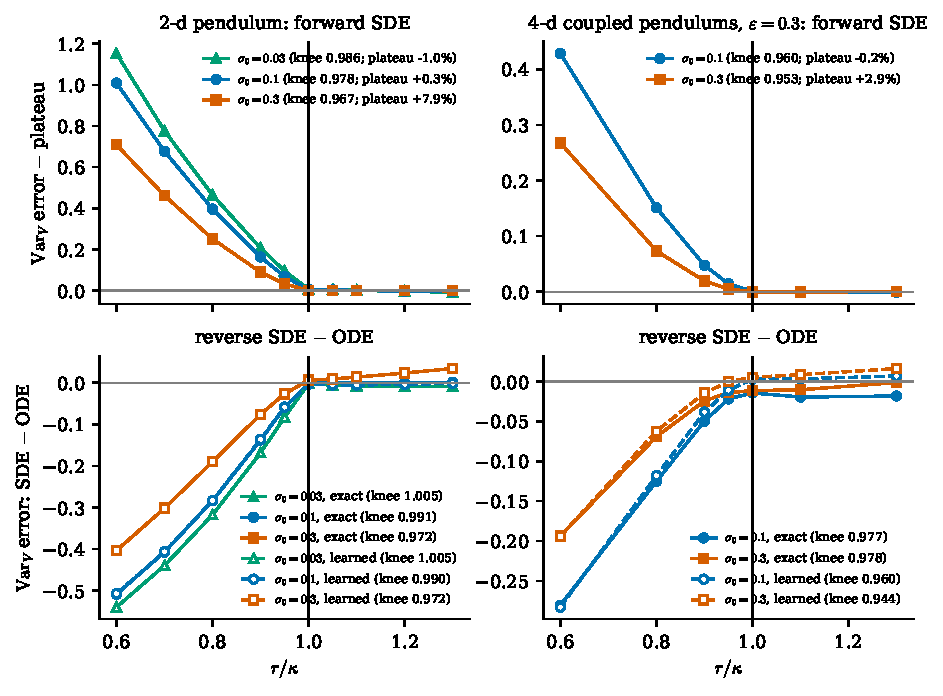
\includegraphics[width=0.9\textwidth]{figures/fig5_knee.pdf}
\caption{Threshold (I) as a function of $r/\kappa$. Top: forward SDE with the physical drift and $G_+$, relative error of the variance along the most stretching direction minus its plateau for $r \geq \kappa$. Bottom: reverse SDE minus probability-flow equation, with exact (filled) and learned (open) scores. Left: pendulum, $\sigma_0 = 0.03$, $0.1$, $0.3$. Right: coupled pendulums, $\varepsilon = 0.3$, $\sigma_0 = 0.1$, $0.3$. The vertical line is $r = \kappa$.}
\label{fig:knee}
\end{figure*}

In four dimensions the exact score is expensive, and the reverse runs used $2000$ paths with the exact score against $20\,000$ with the learned one; the difference between their knees ($0.017$--$0.034$) comes mostly from the small residual offset for $r \geq \kappa$, which differs between the two runs ($-0.011$ to $-0.020$ for the exact score, $+0.003$ to $+0.016$ for the learned one). Measured from the level at $r = \kappa$ instead of from zero, the four knees lie between $0.948$ and $0.964$, within $0.006$ of the shape prediction.
